\documentclass[a4paper, top=10mm]{article}
%for writing from the top
\usepackage{fullpage}
%for math
\usepackage{amsmath}
\usepackage{mathrsfs}
\usepackage{amsthm}
%for images
\usepackage{graphicx}
%for color
\usepackage{xcolor}
%for title
\title{\textbf{\huge{Elves' Sleigh Seats}}}
\author{Enigma n\textsuperscript{o}4}
\date{19\textsuperscript{th} December 2024}

\newtheorem*{hint}{Hint}

\addtolength{\voffset}{-2cm}
\addtolength{\textheight}{5cm}


\begin{document}
	\maketitle
	
	Santa’s sleigh is equipped with 1000 passenger seats, one for each of the 1000 elves who assist Santa in delivering presents. Both the elves and the seats are numbered from 1 to 1000.
	
	When it’s time to board, the first elf (Elf number 1) decides to shake things up and randomly chooses any seat to sit in. After that, the remaining 999 elves board one by one, following these rules:
	
	If their assigned seat (matching their number) is available, they sit in it.
	If their assigned seat is already taken, they pick a random free seat.
	
	When all the elves are seated, what is the probability (expressed as a percentage, rounded to the nearest $0.01\%$) that the last elf (Elf number 1000) ends up sitting in seat number 1000?
	
	\begin{center}
		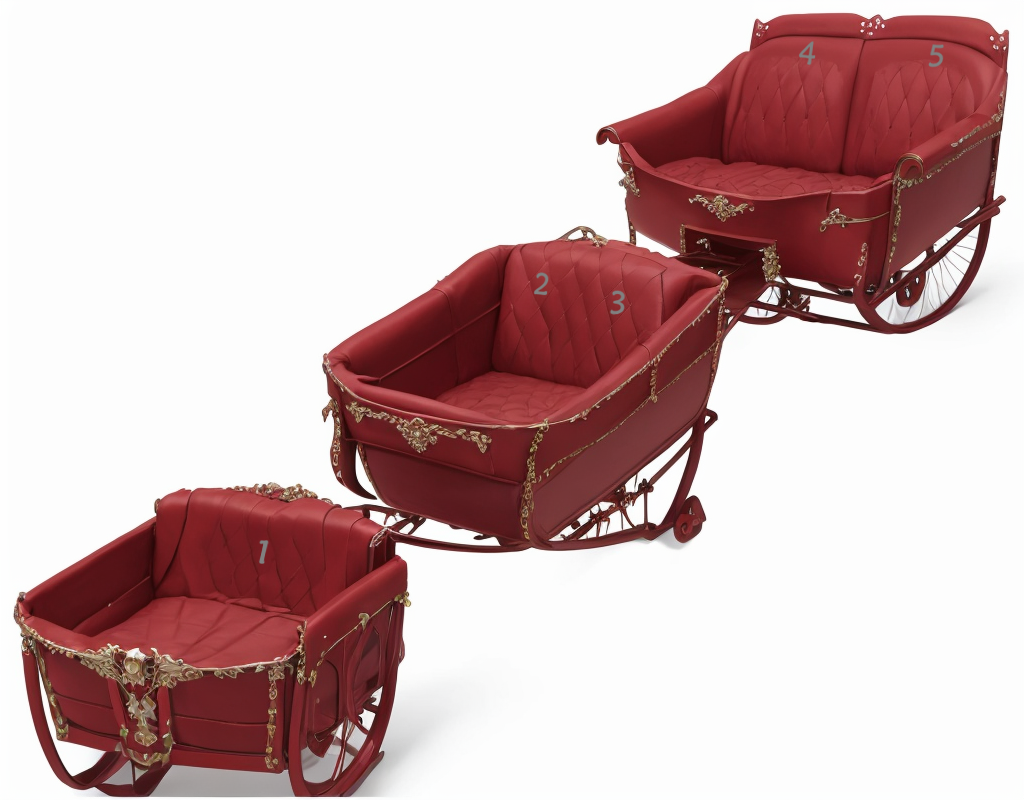
\includegraphics[width=\linewidth]{04sleigh_seats.png}
		Santa's sleigh before elves take their seats.
		
	\end{center}
	
	% Answer: 50%
	
\end{document}